\documentclass[border=5mm]{standalone}
\usepackage{tikz}
\usepackage{xcolor}
\usepackage{pgfplots}

\pgfplotsset{compat=1.18}
\usepgfplotslibrary{statistics}

\usetikzlibrary{shapes,arrows,positioning,backgrounds,calc,intersections,calc}

\definecolor{ugent-re}{RGB}{220, 78, 40}        % vermilion			/ vermiljoen
\definecolor{ugent-we}{RGB}{45, 140, 168}       % no match
\definecolor{ugent-ge}{RGB}{232, 94, 113}       % rose				/ bleekrood
\definecolor{ugent-ea}{RGB}{111, 113, 185}      % distant blue		/ verblauw
\definecolor{ugent-pp}{RGB}{251, 126, 58}       % deep orange		/ dieporanje
\definecolor{ugent-ps}{RGB}{113, 168, 96}       % yellow green		/ geelgroen

\tikzstyle{python}=[fill=ugent-ps!50!white]
\tikzstyle{java}=[fill=ugent-we!50!white]
\tikzstyle{haskell}=[fill=ugent-ea!50!white]
\tikzstyle{js}=[fill=ugent-pp!50!white]
\tikzstyle{c}=[fill=ugent-re!50!white]

\newlength{\block}
\setlength{\block}{0.75cm}

\tikzstyle{a}=[anchor=north west]
\tikzstyle{box}=[a,draw,rectangle]
\tikzstyle{node}=[a,draw,minimum height=0.5cm,align=center,fill=white,text depth=.25ex]
\tikzstyle{document}=[node,tape,tape bend top=none]
\tikzstyle{cont}=[box,minimum height=1\block,minimum width=1\block]
\tikzstyle{arrow}=[draw, -latex]
\tikzstyle{inner}=[box,draw=gray]

% Blue box style
\tikzstyle{bluebox}=[draw=ugent-we,java]
\tikzstyle{redbox}=[draw=ugent-re,c]
\tikzstyle{greenbox}=[draw=ugent-ps,python]

% Some things specific to TESTed imagery.
\tikzstyle{tc}=[box,draw=ugent-ps]
\tikzstyle{comp}=[box,draw=ugent-re,fill=ugent-re,fill opacity=0.05]
\tikzstyle{exec}=[box,draw=ugent-we,fill=ugent-we,fill opacity=0.10]

% Stuff from tested-engine/concept.tex
\tikzstyle{process}=[node,rectangle]
\tikzstyle{terminator}=[node,rectangle,rounded corners=0.5cm]
\tikzstyle{io}=[node,trapezium,trapezium left angle=70,trapezium right angle=-70,minimum width=2.5cm,trapezium stretches=true]
\tikzstyle{small}=[font=\footnotesize,color=darkgray]
\tikzstyle{submission}=[document,align=right,minimum width=3cm,minimum height=1cm,text depth=0.5cm,inner sep=0.5mm,font=\scriptsize]

% Stuff from chatper3/flow.tex
\tikzstyle{height}=[minimum height=0.75\block]
\tikzstyle{contt}=[cont,minimum height=0.75\block]
\tikzstyle{compop}=[comp,text opacity=1]
\tikzstyle{execop}=[exec,text opacity=1]

\tikzstyle{hnode}=[draw,anchor=center,minimum height=\block,text depth=.25ex,align=center]
\tikzstyle{executable}=[hnode,ultra thick,fill=gray!10]
\tikzstyle{inner-exec}=[node,anchor=center,minimum width=3.25\block,densely dotted,font=\footnotesize,fill=none]
\tikzstyle{stmt}=[node,anchor=center,fill=gray!30,minimum width=4.5\block,font=\footnotesize]
\tikzstyle{fieldset}=[minimum height=\block,fill=white,text depth=.5ex,fill=white]
\usepackage{pgfplots}
\usepackage{textcomp}
\pgfplotsset{compat=1.18}
\begin{document}
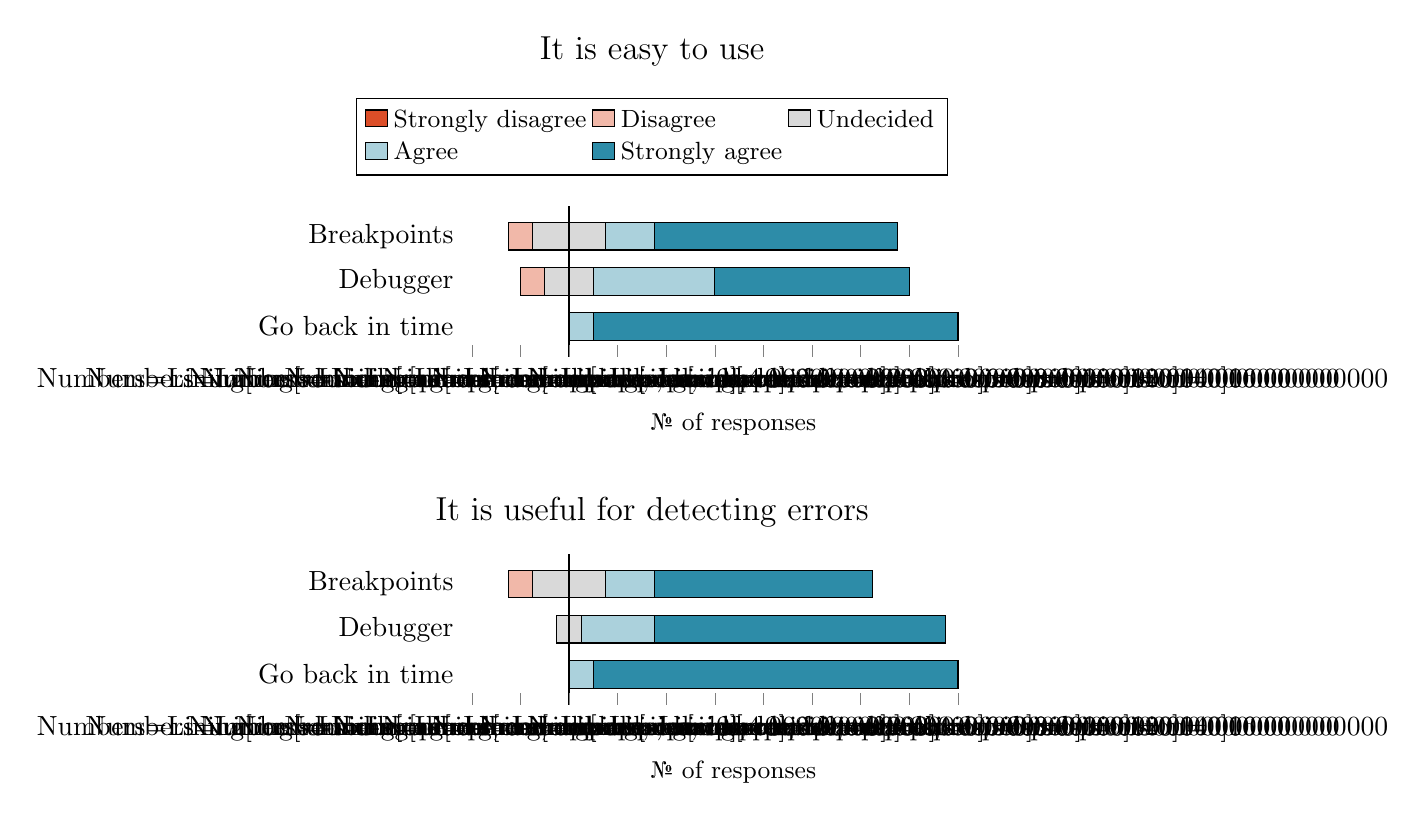
\begin{tikzpicture}
    \pgfplotsset{
        undecided/.style={fill=gray!30},
        sdisagree/.style={fill=ugent-re},
        disagree/.style={fill=ugent-re!40},
        agree/.style={fill=ugent-we!40},
        sagree/.style={fill=ugent-we}
    }
    \begin{axis}[
        name=use,
        title={It is easy to use},
        height=3.5cm,
        width=\axisdefaultwidth,
        xbar stacked,
        symbolic y coords={Go back in time,Debugger,Breakpoints},
        ytick distance=1,
        xtick distance=2,
        extra x ticks={0},
        extra x tick style={
            grid style={black,thick},
            xticklabel=\empty,
            xmajorgrids
        },
        enlarge y limits={abs=11pt},
        axis on top,
        xlabel={\textnumero{} of responses},
        xlabel style={font=\small},
        xtick pos=bottom,
        ytick style={draw=none},
        axis line style={draw=none},
        legend columns=3,
        legend cell align={left},
        legend style={at={(0.35,1.2)},anchor=south,font=\small},
        title style={at={(0.35,1.75)},anchor=south,font=\large},
        xticklabel={\addfontfeature{Numbers={Lining}}\num[round-mode=places, round-precision=0]{\tick}}
    ]
        % Undecided part 1
        \addplot[undecided,forget plot] coordinates {
            (-1.5,Breakpoints)
            (-1,Debugger)
            (-0,Go back in time)
        };
        % Disagree
        \addplot[disagree,forget plot] coordinates {
            (-1,Breakpoints)
            (-1,Debugger)
            (0,Go back in time)
        };
        % Strongly disagree
        \addplot[sdisagree,forget plot] coordinates {
            (0,Breakpoints)
            (0,Debugger)
            (0,Go back in time)
        };
        % Undecided part 2
        \addplot[undecided,forget plot] coordinates {
            (1.5,Breakpoints)
            (1,Debugger)
            (0,Go back in time)
        };
        % Agree
        \addplot[agree,forget plot] coordinates {
            (2,Breakpoints)
            (5,Debugger)
            (1,Go back in time)
        };
        % Strongly agree
        \addplot[sagree,forget plot] coordinates {
            (10,Breakpoints)
            (8,Debugger)
            (15,Go back in time)
        };

        \addlegendimage{fill=ugent-re}
        \addlegendentry{Strongly disagree},
        \addlegendimage{fill=ugent-re!40}
        \addlegendentry{Disagree}
        \addlegendimage{fill=gray!30}
        \addlegendentry{Undecided}
        \addlegendimage{fill=ugent-we!40}
        \addlegendentry{Agree}
        \addlegendimage{fill=ugent-we}
        \addlegendentry{Strongly agree}

    \end{axis}
    \begin{axis}[
        at={($(use.south)+(0cm,-2.5cm)$)},
        anchor=north,
        title={It is useful for detecting errors},
        height=3.5cm,
        width=\axisdefaultwidth,
        xbar stacked,
        symbolic y coords={Go back in time,Debugger,Breakpoints},
        ytick distance=1,
        xtick distance=2,
        extra x ticks={0},
        extra x tick style={
            grid style={black,thick},
            xticklabel=\empty,
            xmajorgrids
        },
        xlabel style={font=\small},
        enlarge y limits={abs=11pt},
        axis on top,
        xlabel={\textnumero{} of responses},
        xtick pos=bottom,
        ytick style={draw=none},
        axis line style={draw=none},
        title style={at={(0.35,1)},anchor=south,font=\large},
        xticklabel={\addfontfeature{Numbers={Lining}}\num[round-mode=places, round-precision=0]{\tick}}
    ]
        % Undecided part 1
        \addplot[undecided,forget plot] coordinates {
            (-1.5,Breakpoints)
            (-0.5,Debugger)
            (0,Go back in time)
        };
        % Disagree
        \addplot[disagree,forget plot] coordinates {
            (-1,Breakpoints)
            (0,Debugger)
            (0,Go back in time)
        };
        % Strongly disagree
        \addplot[sdisagree,forget plot] coordinates {
            (0,Breakpoints)
            (0,Debugger)
            (0,Go back in time)
        };
        % Undecided part 2
        \addplot[undecided,forget plot] coordinates {
            (1.5,Breakpoints)
            (0.5,Debugger)
            (0,Go back in time)
        };
        % Agree
        \addplot[agree,forget plot] coordinates {
            (2,Breakpoints)
            (3,Debugger)
            (1,Go back in time)
        };
        % Strongly agree
        \addplot[sagree,forget plot] coordinates {
            (9,Breakpoints)
            (12,Debugger)
            (15,Go back in time)
        };
    \end{axis}
\end{tikzpicture}
\end{document}
